
\chapter{PEOPLE: Predetermined Order, Prunded Label}

Das erstellen von Abkürzungen während der Kontraktion eines Knotes $v$ erfordert mindestens $\abs{\text{Vorgänger}} \cdot \abs{\text{Nachfolger}}$ viele Vergleiche, ob eine Kante einzufügen ist.
Wird zusätzlich noch für jeden Vorgänge eine Dijkstra Suche ausgeführt, so steigt der Zeitbedarf noch einmal deutlich an
Wird eine Warteschlange mit Kanten-Differenz benutzt, so sind alleine für die Initalsierung deren Initialsierung $\sum_{v \in V} \abs{\text{Vorgänger}(v)} \cdot \abs{\text{Nachfolger}(v)}$ Vergleiche notwendig.
Für Graphen, welche Knoten mit einem hohem Grad enthalten, kann dies dazu führen, dass die Kontraktion mancher Knoten nicht mehr in einem sinvollen Zeitrahmen berechenbar ist.
Trotzdem wäre es praktisch, wenn sich die Query-Zeiten von Contraction Hierarchirs und Hierachical Hub Labeling auch auf sie übertragen ließen.

Um die Nachfolgende Definition vorzubereiten, betrachten wir ein Beispiel.
Sei $G = (V, E)$ mit $\supset V \supset \{ u, v, w \}$ und $E = \{ (u, v, {spd}((u, v))), (v, w, {spd}((v, w))) \}$, ein Produkt einer Kontraktion, also zu Beginn mehr Kanten und nicht-isolierte Knoten entiehlt
Es soll nun $v$ kontraktiert werden.
Hierfür wir eine Kante $(u, w, {spd}((u, w)))$ eingefügt und die Kanten $(u, v), (v, w)$ entfernt.
Was bedeuted dies für den enstehenden Contracted Graph $C$?
\begin{enumerate}
    \item
          Alle Knoten, einschließlich $v$ haben ein niedriges Level als $u$ und $w$.
          Inbesondere haben alle Knoten auf allen kürzesten Pfaden von $u$ nach $w$, also die, die bereits kontraktiert wurden, ein niedrigeres Level.

    \item
          $(u, w) \in E_u$ gilt genau dann, wenn $w$ das größte Level auf allen Pfaden von $u$ nach $w$.
          $(w, u) \in E_d$ gilt, wenn $u$ das größte Level hat.
\end{enumerate}

Es kann nun gezeigt werden, dass auch die Rückrichtung gilt, also dass basienden auf dieser Chracterisierung ein Contracted Graph gebildet werden kann.

% \begin{definition}[max-on-paths]
%     Sei $G = (V, E)$ und ${vtl}$ eine \emph{vertex-to-level} Funktion dazu.
%     Dann ist die \emph{max-on-paths} Funktion ${mop} \colon V \times V \to L$ definiert als größte Level eines Knotens auf allen kürzesten Pfaden zwischen zwei Knoten.
% \end{definition}

\begin{definition}[Upward Graph]\label{people:def:upward_graph}
    Sei $G = (V, E)$ und ${vtl}$ eine \emph{vertex-to-level} Funktion dazu. Dann ist $G_u = (V, E_u)$ ein \emph{upward Graph} zu $G$ wenn gilt:

    Für jeden Knoten $t \in V$ ist $(t, h, {spd}((t, h))) \in E_u$ mit $h \in V$ wenn $h$ das größte und $t$ das zweitgrößte Level auf allen kürzesten Wege auf $G$ von $t$ nach $h$ hat.
\end{definition}

Betrachten wir das ganze an dem bereits definierten Beispielgraph.
Sei ${vtl}$ definiert durch die Abbildung in \autoref{ch::fig::vtl_abbildung} definiert.
Durch Anwendung der Definition \ref{people:def:upward_graph} ergibt sich der in \autoref{ch::fig::upward_graph} gezeigte Upward Graph.

\begin{table}[ht]
    \centering
    \begin{tabular}{lllllllllllll}
        Vertex & a & b & c & d & e & f & g & h & i & j  & k & \\
        Level  & 8 & 7 & 3 & 6 & 2 & 5 & 1 & 4 & 0 & 10 & 9 &
    \end{tabular}
    \caption{${vtl}$ Beispielfunktion}
    \label{ch::fig::vtl_abbildung}
\end{table}


\begin{figure}[ht]
    \centering
    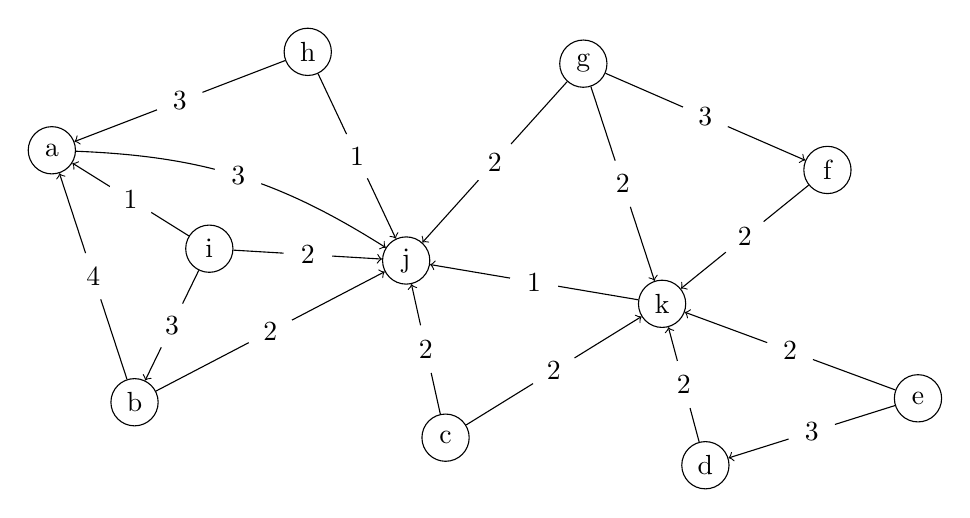
\begin{tikzpicture}
        % Nodes
        \node[circle, draw, minimum size=0.6cm, inner sep=0pt] at (0.5* 0.0, 0.5* 8.5)  (a)    {a};
        \node[circle, draw, minimum size=0.6cm, inner sep=0pt] at (0.5* 2.1, 0.5* 2.1)  (b)    {b};
        \node[circle, draw, minimum size=0.6cm, inner sep=0pt] at (0.5* 10.0, 0.5* 1.2)  (c)    {c};
        \node[circle, draw, minimum size=0.6cm, inner sep=0pt] at (0.5* 16.6, 0.5* 0.5)  (d)    {d};
        \node[circle, draw, minimum size=0.6cm, inner sep=0pt] at (0.5* 22.0, 0.5* 2.2)  (e)    {e};
        \node[circle, draw, minimum size=0.6cm, inner sep=0pt] at (0.5* 19.7, 0.5* 8.0)  (f)    {f};
        \node[circle, draw, minimum size=0.6cm, inner sep=0pt] at (0.5* 13.5, 0.5* 10.7)  (g)    {g};
        \node[circle, draw, minimum size=0.6cm, inner sep=0pt] at (0.5* 6.5, 0.5* 11.0)  (h)    {h};
        \node[circle, draw, minimum size=0.6cm, inner sep=0pt] at (0.5* 4.0, 0.5* 6.0)  (i)    {i};
        \node[circle, draw, minimum size=0.6cm, inner sep=0pt] at (0.5* 9.0, 0.5* 5.7)  (j)    {j};
        \node[circle, draw, minimum size=0.6cm, inner sep=0pt] at (0.5* 15.5, 0.5* 4.6)  (k)    {k};


        \draw[->]  (a) edge[bend left=15] node[circle, fill=white] {3} (j);

        \draw[->]  (b) edge node[circle, fill=white] {4} (a);
        \draw[->]  (b) edge node[circle, fill=white] {2} (j);

        \draw[->]  (c) edge node[circle, fill=white] {2} (j);
        \draw[->]  (c) edge node[circle, fill=white] {2} (k);

        \draw[->]  (d) edge node[circle, fill=white] {2} (k);

        \draw[->]  (e) edge node[circle, fill=white] {3} (d);
        \draw[->]  (e) edge node[circle, fill=white] {2} (k);

        \draw[->]  (f) edge node[circle, fill=white] {2} (k);

        \draw[->]  (g) edge node[circle, fill=white] {3} (f);
        \draw[->]  (g) edge node[circle, fill=white] {2} (j);
        \draw[->]  (g) edge node[circle, fill=white] {2} (k);

        \draw[->]  (h) edge node[circle, fill=white] {3} (a);
        \draw[->]  (h) edge node[circle, fill=white] {1} (j);

        \draw[->]  (i) edge node[circle, fill=white] {1} (a);
        \draw[->]  (i) edge node[circle, fill=white] {3} (b);
        \draw[->]  (i) edge node[circle, fill=white] {2} (j);


        \draw[->]  (k) edge node[circle, fill=white] {1} (j);
    \end{tikzpicture}
    \caption{Upward Graph des Beispielgraphs}
    \label{ch::fig::upward_graph}
\end{figure}

Die Definition des Downward Graphens erfolgt nun analog zu der des Upward Graphens:

\begin{definition}[Downward Graph]
    Sei $G = (V, E)$ und ${vtl} \coloneq V \to \mathbb{N}$ eine \emph{vertex-to-level} Funktion. Dann ist ein upward Graph des Umkehrgraphens $G^T$ ein \emph{downward Graph} zu $G$.
\end{definition}

Wenn ein Graph ungerichtet ist, dann ist er äuivalent zu seinem Umkehrgraphen und dann ist auch der Upward und Downward Graph äuivalent.
Daher entspricht \autoref{ch::fig::upward_graph} gleichzeitig auch dem Downward Graph des Beispielgraphens.


